\RequirePackage{luatex85,shellesc}
\documentclass[tikz,multi=false]{standalone}
\usepackage{pgfplots}
\usepackage{ifthen}
\usepackage{xstring}
\usepackage[sfdefault]{FiraSans}
\usepackage{eulervm}
\usepackage{circuitikzgit}
\usepackage{pgfplots}
\usetikzlibrary{calc,graphs,graphdrawing,fit,positioning}
\usetikzlibrary{decorations,decorations.footprints,decorations.shapes}
\usetikzlibrary{shapes,arrows,arrows.meta}
\usetikzlibrary{arrows,arrows.meta}
\usetikzlibrary{calc,positioning,fit,shapes}
\usegdlibrary{layered}
\usepackage{xstring}
\pgfplotsset{compat=1.15}

\begin{document}

% \CAMKIIRING{label}{x}{y}{list_of_phosphorylated_subunits}{radius_of_subunit}{no_of_subunits}


\newcommand{\tstar}[5]{% x, y, inner radius, outer radius, tips,
    \pgfmathsetmacro{\starangle}{360/#5}
    \draw[draw=none,fill=blue!40] [xshift=#1cm,yshift=#2cm](0:#3)
    \foreach \x in {1,...,#5}
    { -- (\starangle/2+\x*\starangle-\starangle/2:#4) -- (#4+\x*\starangle:#3)
    }
    -- cycle;
}

\newcommand{\TSTAR}[3]{% pos, radius, tips,
    \node[star,star points=#3,star point ratio=0.3,fill=blue!40,minimum
    size=#2cm,] (inner#3) at (#1) {};
}


\newcommand{\CAMKIIRING}[6] { % name, x, y, indices_of_red_balls, size, tips 
    % get the theta for given number of subunits.
    \pgfmathsetmacro{\theta}{360/#6};
    \pgfmathsetmacro{\r}{0.5*#5/sin(\theta/2)};
    \tstar{#2}{#3}{\r/5}{\r}{#6};
    \begin{scope}[ ]
        \def\fitlist{};
        \foreach \i in {1,...,#6}
        {
            \IfSubStr {#4} {\i}
            {
                \node[ball color=red,circle,shading=ball,minimum size=#5cm] (r\i) at
                ($(\i*\theta:\r cm)+(#2,#3)$) {};
            }
            {
                \node[draw=none,ball color=blue,circle,minimum size=#5cm](r\i) at
                ($(\i*\theta:\r cm)+(#2,#3)$) {}; 
            }
            \xdef\fitlist{\fitlist(r\i)};
        };
        % inner subunit.

        \node[circle,fit=\fitlist,] (#1) {};
        %\node[] at (#2,#3) {#1};
    \end{scope}
}

\newcommand\SUBUNIT[4]{ % name, pos, radius, color
    \node[draw=none,ball color=#4,inner sep=0,circle,minimum size=#3 cm] (#1) at #2 {}; 
}

\newcommand{\CAMKII}[5] { % name, position, indices_of_red_balls, size, tips 
    % get the theta for given number of subunits.
    \node (#1) at (#2) {};
    \begin{scope}[ ]
        \pgfmathsetmacro{\theta}{360/#5};
        \pgfmathsetmacro{\r}{0.5*#4/sin(\theta/2)};
        \def\fitlist{};

        \node[draw=none] (#1_root) at (#1) {};
        % inner subunit.
        \TSTAR{#1_root.center}{0.4*\r}{#5};

        \foreach \i in {1,...,#5}
        {
            \IfSubStr {#3} {\i}
            {
                \node[draw=none,inner sep=0,ball color=red,circle,minimum size=#4cm] (r\i) at
                ($(\i*\theta:\r cm)+(#1_root)$) {};
            }
            {
                \node[draw=none,ball color=blue,inner sep=0,circle,minimum size=#4cm](r\i) at
                ($(\i*\theta:\r cm)+(#1_root)$) {}; 
            }
            \xdef\fitlist{\fitlist(r\i)};
        };
        \node[fit=\fitlist,circle,inner sep=0] (#1) {};
    \end{scope}
}

\newcommand{\CAMKIIWithoutHub}[5] { % name, position, indices_of_red_balls, size, tips 
    % get the theta for given number of subunits.
    \node (#1) at (#2) {};
    \begin{scope}[ ]
        \pgfmathsetmacro{\theta}{360/#5};
        \pgfmathsetmacro{\r}{0.5*#4/sin(\theta/2)};
        \def\fitlist{};

        \node[draw=none] (#1_root) at (#1) {};

        \foreach \i in {1,...,#5}
        {
            \IfSubStr {#3} {\i}
            {
                \node[draw=none,inner sep=0,ball color=red,circle,minimum size=#4cm] (r\i) at
                ($(\i*\theta:\r cm)+(#1_root)$) {};
            }
            {
                \node[draw=none,ball color=blue,inner sep=0,circle,minimum size=#4cm](r\i) at
                ($(\i*\theta:\r cm)+(#1_root)$) {}; 
            }
            \xdef\fitlist{\fitlist(r\i)};
        };
        \node[fit=\fitlist,circle,inner sep=0] (#1) {};
    \end{scope}
}


\newcommand{\CACAM}[3] { % name, (x, y), size 
    % A node is created with given name which fit all others.
    \node (#1) at (#2) { };
    \edef\name{#1_center}
    \begin{scope}[]
        \pgfmathsetmacro{\car}{#3/2}
        \node[star,star points=4,fill=red,minimum size=#3 cm,inner sep=0pt] 
            (\name) at (#1) {};

        \foreach \x in {1,...,4} 
        {
            \pgfmathsetmacro{\theta}{360/4*\x};
            \node[inner sep=0pt,ball color=yellow,circle,minimum size=\car cm] 
            (ca\x) at ($(#2)+(\theta:\car cm)$) {};
        }
        \node[circle,inner sep=0,fit=(ca1) (ca2) (ca3) (ca4) (\name)] (#1)  {};
    \end{scope}
}

\newcommand{\CAM}[3] { % name, (x, y), size 
    \node (#1) at (#2) { };
    \begin{scope}[]
        \pgfmathsetmacro{\car}{#3/2}
        \node[star,star points=4,star point ratio=2
            , fill=red,minimum size=#3 cm,inner sep=0pt] 
            (rcam) at (#1) {};
    \end{scope}
}

% NMDA receptors and other.
% \NMDAOLD}{(x,y)}{width}{gap}{rotation}
\newcommand{\NMDAOLD}[5] {
    \pgfmathsetmacro\rwidth{#3/5.0}
    \pgfmathsetmacro\gap{0.1+#4}

    \edef\ang{#5}
    \node[minimum height=#3 cm,minimum width=\gap cm] (#1) at #2 {};
    \begin{scope}[rotate around={(\ang:#2)}]
        \foreach \xshift/\name in {\gap/#1_right,-\gap/#1_left}
        {
            \node[draw=blue,fill=red!20,rectangle, inner sep=0pt
                , decorate, decoration={random steps,amplitude=1pt,segment length=1pt}
                , minimum height=#3cm ,minimum width=\rwidth cm
            ] (\name) at ([xshift=\xshift cm]#1.east) {};
        }
    \end{scope}
}

% \AMPA{name}{(x0,y0)}{height}{gap or opening size}{rotation}
\newcommand{\AMPA}[5] {
    \pgfmathsetmacro{\rwidth}{#3/5.0}
    \pgfmathsetmacro\rwidth{#3/5.0}
    \pgfmathsetmacro\gap{0.1+#4}
    \edef\ang{#5}

    \node (#1) at #2 {};
    \begin{scope}[rotate around={(\ang:#2)}]
        \foreach \i in {\gap,0}
        {
            \node[minimum height=#3 cm,minimum width=\gap cm
                ,transform shape   % necessary when within scope
                ,cylinder,fill=red
            ] (#1_\i) at ([yshift=\i cm]#1) {};
        }
    \end{scope}
}

% \CA{label}{coordinate}{label}
\newcommand{\CA}[3] {
    \node (#1) at #2 {};
    \node[shading=ball,circle,ball color=yellow,inner sep=0,minimum size=2 mm]
        at (#1) { };
}


%%%%%%%%%%%%%%%%%%%%%%%%%%%%%%
%% Chemical equilibrium arrow 

\newdimen\arrowsize
\newdimen\mylw
\pgfkeys{/my arrows/chemeq/.style={draw,thick,double distance=3pt,onearc-onearc}}
\pgfkeys{/my arrows/size/.code={\pgfsetarrowoptions{onearc}{#1}}}
\def\myalw{1pt}
\pgfarrowsdeclare{onearc}{onearc}{%
  \mylw=\myalw
  \pgfarrowsleftextend{-\pgfgetarrowoptions{onearc}-.5\mylw}
  \pgfarrowsrightextend{1pt}
}{%
  \pgfsetdash{}{0pt}
  \mylw=\pgflinewidth
  \pgfsetlinewidth{\myalw}
  \advance\arrowsize by.5\pgflinewidth
  \pgfpathmoveto{\pgfpoint{-\pgfgetarrowoptions{onearc}}{-\pgfgetarrowoptions{onearc}-.5\mylw}}%
  \pgfpatharc{180}{90}{\pgfgetarrowoptions{onearc}}
  \pgfusepathqstroke
}


%  \PHOSPHO{name}{location}
\newcommand\PHOSPHO[2]
{
    \node[circle,fill=yellow,inner sep=0pt] (#1) at (#2) {\tiny P};
}


\newcommand{\CAMKIIHOLOENZYME}[6] { % name, x, y, indices_of_red_balls, size, tips 
    % get the theta for given number of subunits.
    \begin{scope}[ ]
        \pgfmathsetmacro{\theta}{360/#6};
        \pgfmathsetmacro{\r}{0.5*#5/sin(\theta/2)};
        \def\fitlist{};
        \foreach \i in {1,...,#6}
        {
            \IfSubStr {#4} {\i}
            {
                \node[ball color=red,circle,shading=ball,minimum size=#5cm] (r\i) at
                ($(\i*\theta:\r cm)+(#2,#3,0)$) {};
            }
            {
                \node[draw=none,ball color=blue,circle,minimum size=#5cm](r\i) at
                ($(\i*\theta:\r cm)+(#2,#3,0)$) {}; 
            }
            \xdef\fitlist{\fitlist(r\i)};
        };

        % inner hub.
        % \tstar{#2}{#3}{\r/5}{\r}{#6};

        \foreach \i in {1,...,#6}
        {
            \IfSubStr {#4} {\i}
            {
                \node[ball color=red,circle,shading=ball,minimum size=#5cm] (r\i) at
                ($(\i*\theta:\r cm)+(#2,#3,\r)$) {};
            }
            {
                \node[draw=none,ball color=blue,circle,minimum size=#5cm](r\i) at
                ($(\i*\theta:\r cm)+(#2,#3,\r)$) {}; 
            }
            \xdef\fitlist{\fitlist(r\i)};
        };
        \node[circle,fit=\fitlist,] (#1) {};
        %\node[] at (#2,#3) {#1};
    \end{scope}
}



\newcommand\SWITCH[6]{ % name, x, y, width, rotation, on-off
    \edef\y{0.2}
    \ifthenelse{#6=1}{\edef\y{0.1}}{}
    \begin{scope}[xshift=-#2, yshift=-#3, rotate=#5]
        \draw[-Circle,line width=#4] (0 cm,0 cm) node (#1_a) {} -- (1 cm,0);
        \draw[Circle-,line width=#4] (1.5 cm,0) -- (2.5 cm,0) node (#1_b) {};
        \draw[line width=#4] (1 cm,\y cm) -- (1.5 cm,\y cm);
        \draw[line width=#4] (1.25 cm,\y cm) -- ++(0,0.2 cm);
    \end{scope}
}

%%%%%%%%%%%%%%%%%%%%%%%%%%%%%%
%% Chemical equilibrium arrow 

\newdimen\arrowsize
\newdimen\mylw
\pgfkeys{/my arrows/chemeq/.style={draw,thick,double distance=3pt,onearc-onearc}}
\pgfkeys{/my arrows/size/.code={\pgfsetarrowoptions{onearc}{#1}}}
\def\myalw{1pt}
\pgfarrowsdeclare{onearc}{onearc}{%
  \mylw=\myalw
  \pgfarrowsleftextend{-\pgfgetarrowoptions{onearc}-.5\mylw}
  \pgfarrowsrightextend{1pt}
}{%
  \pgfsetdash{}{0pt}
  \mylw=\pgflinewidth
  \pgfsetlinewidth{\myalw}
  \advance\arrowsize by.5\pgflinewidth
  \pgfpathmoveto{\pgfpoint{-\pgfgetarrowoptions{onearc}}{-\pgfgetarrowoptions{onearc}-.5\mylw}}%
  \pgfpatharc{180}{90}{\pgfgetarrowoptions{onearc}}
  \pgfusepathqstroke
}

\newcommand\PreSynSide[1]{%name
    % Draw pre synaptic side.
    % Draw synapse. Pre synaptic side.
    \begin{scope}[rotate=180, local bounding box=#1]
        \draw[color=red!30,very thick, fill=red!10] plot[smooth] coordinates { 
            (-3,-5) (-3,-4) (-6,-2) (-7,1) 
            (0,1) (3,1) (2.5,-2) (-1,-4) 
            (-1,-5) 
        };
    \end{scope}

    \begin{scope}[rotate=-90]
        % Pre synaptic side fill-in.
        \tikzset{every path/.style={line width=3pt,dashed}}
        \tikzset{pre/.style={-{o[width=5pt]},very thick}}

        \foreach[count=\i] \j in {1,3,5,7,9,11}
        {
            \draw[pre,color=blue!20] plot[smooth] coordinates { 
                (-5+0.1*rnd,1.4+0.1*\j) 
                (-4+0.1*rnd,1.15+0.15*\j)
                (-3+0.1*rnd,-1.5+0.55*\j)
                (-2+0.1*rnd,-2.5+0.75*\j)
                (-1+0.1*rnd,-3+0.85*\j)
                (0+0.1*rnd,-3.3+0.9*\j)
                (1+0.1*rnd,-3.4+0.9*\j)
            };
        }
    \end{scope}
}

\newcommand\PostSynSide[1]{%name
    % Draw pre synaptic side.
    % Draw synapse. Pre synaptic side.
    \begin{scope}[rotate=0, local bounding box=#1, xshift=4cm, yshift=-3cm]
        \draw[color=red!30,very thick, fill=red!10] plot[smooth] coordinates { 
            (-3,-5) (-3,-4) 
            (-6,-2.5) 
            (-7,1) (0,1) (3,1) 
            (2.5,-2.5) 
            (-1,-4) (-1,-5) 
        };
    \end{scope}
}



\begin{tikzpicture}[scale=1]

    \PreSynSide{preA}
    \PostSynSide{postA}
    \node[rotate=0, scale=1] (camkii) at (postA) 
    {
        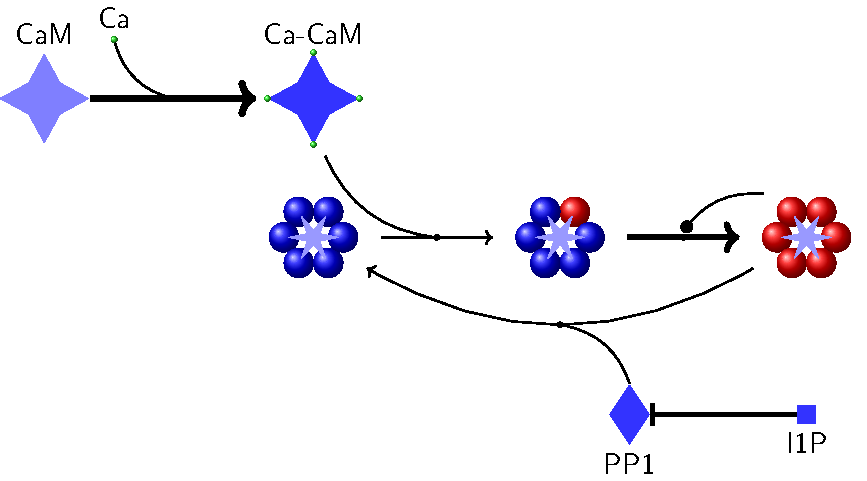
\includegraphics[width=5cm]{../elifeFigure1/camkii_pp1_switch_level1_detail.pdf}
    };
    \node[rotate=0, scale=1, above=0cm of camkii] (se) 
    {
        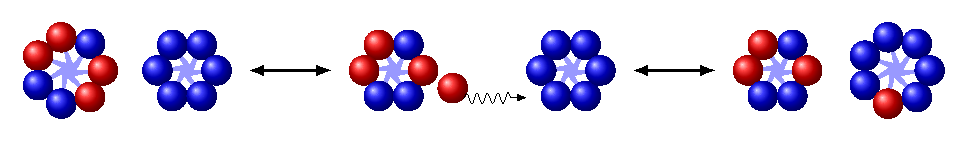
\includegraphics[width=5cm]{../elifeFigure1/camkii_subunit_exchange.pdf}
    };

\end{tikzpicture}	
\end{document}

